\section{Среднеквадратичная аппроксимация (дискретный случай). Понятие веса.}\label{sec:ch13}
Критерий интерполирования, предполагающий совпадение исходной и аппроксимирующей функции в узлах таблицы, не является
единственным. Обратимся к экспериментальным данным, представленным на рисунке (а).
\begin{figure}[H]
    \centering
    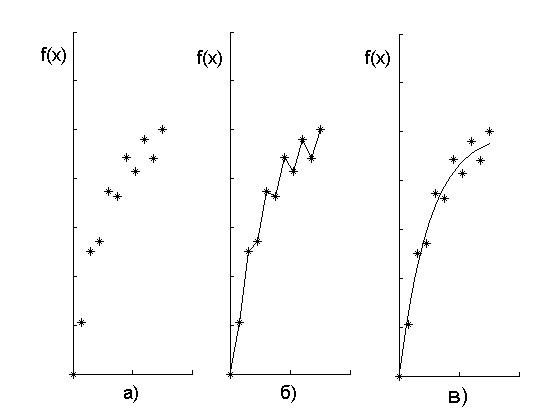
\includegraphics[width=0.5\linewidth]{subfiles/images/13_1}
\end{figure}
Если выполнить по ним интерполяцию, то получится кривая на рис. (б). Маловероятно, чтобы ее вид отвечал исходной
зависимости, положенной в основу таблицы. Вероятнее всего, что этой зависимости отвечает кривая, похожая на рис. (в),
а отклонение экспериментальных данных от нее продиктовано сравнительно большой погрешностью измерений. В таком случае
целесообразно использовать среднеквадратичный критерий
\begin{equation*}
    \rho^2 = \sum_{k=1}^{N} \left( f(x_k) - g(x_k) \right)^2
\end{equation*}
или, если аппроксимируемая функция задана непрерывно,
\begin{equation*}
    \rho^2 = \int_a^b \left( f(x_k) - g(x_k) \right)^2 dx
\end{equation*}

Близость функций по среднеквадратичному критерию еще не гарантирует малой величины их максимальной разности
\begin{equation*}
    \delta = \max_{[a, b]} \left| f(x) - g(x) \right|
\end{equation*}
Малое значение интеграла или суммы свидетельствует лишь о том, что почти на всем отрезке $[a, b]$ значения $f(x)$ и $g(x)$
мало отличаются друг от друга, хотя в отдельных точках или на небольших отрезках разность их значений может быть
значительной.

Проблема выбора аппроксимирующей функции решается так же, как и при интерполяции: $Q(x)$ выбирается в виде обобщенного
многочлена:
\begin{equation}
    Q_m(x) = \sum_{k=0}^{m} a_k \varphi_k (x) \label{eq:com_polynom}
\end{equation}
где $\left\{ \varphi_k \right\}$ -- заданный набор линейно независимых функций, а коэффициенты $a_k$ подлежат определению.

\subsection{Дискретный случай. Весовые коэффициенты.}
Функция $f(x)$ задается на дискретном множестве точек таблицей, а ее аппроксимация $Q_m(x)$ выбирается в виде обобщенного
многочлена~\eqref{eq:com_polynom}. Коэффициенты $a_k$ выбираются из условия минимума величины $\rho^2$
\begin{equation}
    \rho^2 = \sum_{i=1}^{N} \left( Q_m(x_i) - f(x_i) \right)^2 \rightarrow \min \label{eq:approx_criteria}
\end{equation}
Рассмотрим три варианта соотношения $N$ и $m$.
\begin{enumerate}
    \item $N = m + 1$

    Число коэффициентов $a_k$ равно числу точек таблицы, решение задачи единственное, и им является интерполяционный
    полином, проходящий через все точки. Минимальное значение $\rho^2 = 0$.
    \item $N < m + 1$

    Минимальное значение $\rho^2$ также равно нулю, но задача имеет бесконечное множество решений.
    \item $N > m + 1$

    Это типичный случай среднеквадратичной аппроксимации. Более того, на практике часто $N \gg m + 1$. Минимальное
    значение $\rho^2$ оказывается уже, как правило, ненулевым, а задача имеет единственное решение. Рассмотрим этот вариант
    подробнее.
\end{enumerate}
Записываем необходимое условие экстремума
\begin{equation*}
    \frac{\partial \rho^2}{\partial a_k} = 0, \qquad k=0,1,\dots,m
\end{equation*}
и выполняем операцию дифференцирования:
\begin{equation*}
    \frac{\partial \rho^2}{\partial a_k} = 2 \sum_{i=1}^{N} \left( Q_m(x_i) - f(x_i) \right)\varphi_k(x_i) = 0
\end{equation*}
Подставляя в получившуюся формулу выражение для $Q_m(x)$, получаем систему линейных алгебраических уравнений
относительно $a_k$:
\begin{equation}
    \label{eq:approx_eqsys}
    a_0 \sum_{i=1}^{N} \varphi_0(x_i)\cdot \varphi_k(x_i) + a_1 \sum_{i=1}^{N} \varphi_1(x_i)\cdot \varphi_k(x_i) + \dots + a_m \sum_{i=1}^{N} \varphi_m(x_i) \cdot \varphi_k(x_i) = \sum_{i=1}^{N} f(x_i) \cdot \varphi_k(x_i)
\end{equation}

Если определитель системы~\eqref{eq:approx_eqsys} не равен нулю, задача имеет единственное решение. Самой популярной
является аппроксимация полиномами, когда $\varphi_k(x) = x^k$, а система~\eqref{eq:approx_eqsys} принимает вид
\begin{gather*}
    \left( \sum_{i=1}^{N} 1 \right)a_0 + \left( \sum_{i=1}^{N} x_i \right)a_i + \dots + \left( \sum_{i=1}^{N} x^m \right) = \left( \sum_{i=1}^{N} f(x_i) \right)\\
    \left( \sum_{i=1}^{N} x_i \right)a_0 + \left( \sum_{i=1}^{N} x_i^2 \right)a_i + \dots + \left( \sum_{i=1}^{N} x^{m+1} \right) = \left( \sum_{i=1}^{N} f(x_i)x_i \right)
\end{gather*}
\begin{equation}
    \dots
\end{equation}
\begin{equation*}
    \left( \sum_{i=1}^{N} x_i^m \right)a_0 + \left( \sum_{i=1}^{N} x_i^{m+1} \right)a_i + \dots + \left( \sum_{i=1}^{N} x^{2m} \right) = \left( \sum_{i=1}^{N} f(x_i)x_i^m \right)
\end{equation*}

При выполнении среднеквадратичной аппроксимации (другое название -- <<метод наименьших квадратов>>) возможна ситуация,
когда исходные данные имеют различную точность. Если к каким-либо экспериментальным значениям доверие выше, т.е. они
являются более надежными по сравнению с другими, это может быть учтено введением в критерий~\eqref{eq:approx_criteria}
положительных весовых коэффициентов $p_i$.
\begin{equation}
    \rho^2 = \sum_{i=1}^{N} p_i \left( Q_m(x_i) - f(x_i) \right)^2 \rightarrow \min \label{eq:approx_with_p}
\end{equation}

Для тех точек, степень доверия к которым выше, и к которым аппроксимирующую кривую желательно провести ближе, чем к
другим точкам, весовые коэффициенты следует задавать больше. Величину $\rho^2$ можно трактовать, как своеобразную <<функцию
штрафа>>. За отклонение $Q_m(x)$ от $f(x)$ в точке $x_i$ к значению $\rho^2$ добавляется слагаемое (<<штраф>>)
$\left( Q(x_i) - f(x_i) \right)^2$ тем большее, чем больше это отклонение. Если какая-то точка является более
приоритетной и к ней аппроксимирующую кривую желательно провести ближе, с помощью весового коэффициента за отклонение в
этой точке <<штраф>> должен быть увеличен.

На практике положительные весовые коэффициенты $p_i$ часто задают так, чтобы их сумма была равна, например, единице или
100. Последнее часто удобно, но не обязательно. Если все коэффициенты умножить на одно и то же число, то, хотя, $\rho^2$ и
изменится, решение задачи останется прежним. Важным являются отношения $p_i$ друг к другу.
